下面的命题说明如何借助矩阵化与矩阵乘积来表示模 $n$ 乘积。
\begin{proposition}
设 $\Xt\in\RR^{d_1\times\dots\times d_N}$ 且 $\Mb\in\RR^{m\times d_n}$，则 
$(\Xt\ttm n \Mb)_{(n)} = \Mb\Xt_{(n)}$.
\begin{proof}
我们用一张简单的张量网络图来说明特殊情形 $n=2$、$N=3$ 下的这一恒等式，一般情形的推广是直接的。于是
\begin{align*}
(\Xt\ttm2\Mb)_{(2)} 
&= 
\left(
    \begin{tikzpicture}[baseline=\baseline]
    \tikzset{tensor/.style = {minimum size = 0.5cm,shape = circle,thick,draw=black,inner sep = 0pt}, edge/.style = {thick,line width=.4mm},every loop/.style={}}
    \def\y{0}
    \def\x{0}
    \node[tensor,fill=green!50!red!50!white] (At) at (\x,\y){\scalebox{0.85}{$\Xt$}};
    \node[tensor,fill=blue!20!white] (M) at (\x-1,\y) {$\Mb$};
    \draw[edge] (At) -- (M) node [midway,above]
    {\scalebox{0.7}{\dimcolor{$d_2$}}};
    \draw[edge] (M) -- (\x-1.7,\y) node [midway,above]
    {\scalebox{0.7}{\dimcolor{$m$}}};);
    \draw[edge] (At)-- (\x+0.5,\y+0.5) node [below] {\scalebox{0.7}{\dimcolor{$d_1$}}};
    \draw[edge] (At)-- (\x+0.5,\y-0.5) node [above] {\scalebox{0.7}{\dimcolor{$d_3$}}};
    \end{tikzpicture}
\right)_{(2)}
=
    \begin{tikzpicture}[baseline=\baseline]
    \tikzset{tensor/.style = {minimum size = 0.5cm,shape = circle,thick,draw=black,inner sep = 0pt}, edge/.style = {thick,line width=.4mm},every loop/.style={}}
    \def\y{0}
    \def\x{0}
    \node[tensor,fill=green!50!red!50!white] (At) at (\x,\y){\scalebox{0.85}{$\Xt$}};
    \node[tensor,fill=blue!20!white] (M) at (\x-1,\y) {$\Mb$};
    \draw[edge] (At) -- (M) node [midway,above]
    {\scalebox{0.7}{\dimcolor{$d_2$}}};
    \draw[edge] (M) -- (\x-1.7,\y) node [midway,above]
    {\scalebox{0.7}{\dimcolor{$m$}}};);
    \draw[edge] (\x+0.15,\y+0.2)-- (\x+0.5,\y+0.2)-- (\x+0.5,\y+0.05) -- (\x+1,\y+0.05) node [above] {\scalebox{0.7}{\dimcolor{$d_1$}}};
    \draw[edge] (\x+0.15,\y-0.2) -- (\x+0.5,\y-0.2)--(\x+0.5,\y-0.04)--(\x+1,\y-0.04) node [below] {\scalebox{0.7}{\dimcolor{$d_3$}}};
    \end{tikzpicture}\\
&=
\Mb\Xt_{(2)} \in\RR^{m\times d_1d_3}.
\end{align*}
\end{proof}
\end{proposition}
\item\textbf{模-n 乘积~（向量）。} 张量 $\Xt\in\RR^{d_1\times\cdots\times d_N}$ 与向量 $\vb\in\RR^{d_n}$ 的模 $n$ 乘积记作
$\Xt \ttm n \vb \in\RR^{d_1\times\cdots \times d_{n-1}\times d_{n+1}\times \cdots\times d_N}$。注意结果是一个 $N-1$ 阶张量，用张量网络图可表示为 
    $$
\Xt\ttm n \vb
=
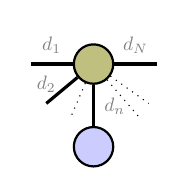
\begin{tikzpicture}[baseline=-0.5ex]
    \tikzset{tensor/.style = {minimum size = 0.5cm,shape = circle,thick,draw=black,inner sep = 0pt}, edge/.style = {thick,line width=.4mm},every loop/.style={}}
    \def\x{6}
    \node[tensor,fill=blue!20!white] (M) at (\x,-1.05) {$\vb$};
    \node[tensor,fill=green!50!red!50!white] (At) at 
    (\x,0) {$\Xt$};
    \draw[edge] (At) -- (\x-0.8,0) node [midway,above] {\scalebox{0.7}{\textcolor{gray}{$d_1$}}};
    \draw[edge] (At)-- (\x-0.6,-0.5) node [above]{\scalebox{0.7}{\textcolor{gray}{$d_2$}}};
    \draw[edge] (At) -- (\x+0.8,0) node [midway,above] {\scalebox{0.7}{\textcolor{gray}{$d_N$}}};;
    \draw[dotted] (At) -- (\x-0.3,-0.7);
    \draw[edge] (At) -- (\x,-0.8) node [midway,right] {\scalebox{0.7}{\textcolor{gray}{$d_n$}}};
    \draw[dotted] (At) -- (\x+0.6,-0.7);
    \draw[dotted] (At) -- (\x+0.7,-0.5);
    \end{tikzpicture}
\in\RR^{d_1\times  \dots\times d_{n-1}\times d_{n+1}\times \dots\times d_N}.
$$
注意，与模 $n$ 矩阵乘法不同，模 $n$ 向量乘法的相乘顺序会影响结果：向量收缩把张量的阶减 1，其后的模指标随之平移。设 $\Xt\in\RR^{d_1\times\cdots\times d_m\times\cdots\times d_n\times\cdots\times d_N}$ 且 $\ab\in\RR^{d_n},\bb\in\RR^{d_m}$，则
$
\Xt\ttm n \ab\ttm m\bb \neq
(\Xt \ttm m \bb)\ttm{n}\ab,
$
因为模 $n$ 向量乘法会去掉第 $m$ 维~\citep{bader2006algorithm}。
\end{enumerate}







下面介绍张量推导中常用的几种乘积：Kronecker 积、Khatri-Rao 积与 Hadamard 积。

\paragraph{Kronecker 积}\label{subsection-kron}
设 $\Ab\in\RR^{m\times n}$、$\Bb\in\RR^{p\times q}$。Kronecker 积 $\Ab\kron\Bb\in\RR^{mp\times nq}$ 定义为
\begin{align}
    \Ab\kron\Bb = 
    \begin{bmatrix}
    a_{11}\Bb & a_{12}\Bb & \dots & a_{1n}\Bb \\
    a_{21}\Bb & a_{22}\Bb & \dots & a_{2n}\Bb \\
    \vdots & \vdots & \ddots & \vdots \\
    a_{m1}\Bb & a_{m2}\Bb & \dots & a_{mn}\Bb 
    \end{bmatrix}.
\end{align}

在张量网络中，Kronecker 积由下图给出：
\begin{align}
    \Ab\kron\Bb = 
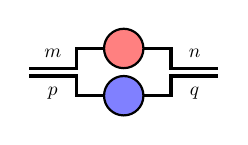
\begin{tikzpicture}[baseline=-0.5ex]
    \tikzset{tensor/.style = {minimum size = 0.5cm,shape = circle,thick,draw=black,inner sep = 0pt}, edge/.style   = {thick,line width=.4mm}}
    \def\x{0}
    \def\y{0}
    \node[tensor,fill=red!50!white] (A) at (\x,\y+0.3){$\Ab$};
    \node[tensor,fill=blue!50!white] (B) at (\x,\y-0.3){$\Bb$};
    \draw[edge] (\x-0.25,\y+0.3) -- (\x-0.6,\y+0.3) -- (\x-0.6,\y+0.05)   -- (\x-1.2,\y+0.05) node [midway,above] {\scalebox{0.7}{\dimcolor{$m$}}};
    \draw[edge] (\x-0.25,\y-0.3) -- (\x-0.6,\y-0.3) -- (\x-0.6,\y-0.05) -- (\x-1.2,\y-0.05) node [midway,below] {\scalebox{0.7}{\dimcolor{$p$}}};
    \draw[edge] (\x+0.25,\y+0.3) -- (\x+0.6,\y+0.3) -- (\x+0.6,\y+0.05) -- (\x+1.2,\y+0.05) node [midway,above] {\scalebox{0.7}{\dimcolor{$n$}}};
    \draw[edge] (\x+0.25,\y-0.3) -- (\x+0.6,\y-0.3) -- (\x+0.6,\y-0.05) -- (\x+1.2,\y-0.05) node [midway,below] {\scalebox{0.7}{\dimcolor{$q$}}};
\end{tikzpicture}.
\end{align}
从这张图可以看出，两个矩阵的 Kronecker 积不过是它们外积的一次重排。事实上，容易验证外积 $\Ab \outprod \Bb$ 的每个分量 $a_{i,j}b_{k,l}$ 都出现在 $\Ab \kron \Bb$ 中；外积是四阶张量，而 Kronecker 积是它的一种矩阵化。更精确地，可以证明 $\Ab \kron \Bb = (\Ab \outprod \Bb)_{(\{1,3\})}$，但我们不在此展开，而是相信张量网络图给出的简洁直观的看法：把 $\Ab$ 与 $\Bb$ 的行腿归到一侧、列腿归到另一侧，所得的矩阵就称为 $\Ab$ 与 $\Bb$ 的 Kronecker 积：
$$\Ab\outprod \Bb =    
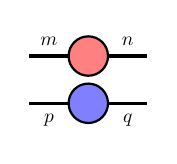
\begin{tikzpicture}[baseline=-0.5ex]
    \tikzset{tensor/.style = {minimum size = 0.5cm,shape = circle,thick,draw=black,inner sep = 0pt}, edge/.style   = {thick,line width=.4mm}}
    \def\x{0}
    \def\y{0}
    \node[tensor,fill=red!50!white] (A) at (\x,\y+0.3){$\Ab$};
    \node[tensor,fill=blue!50!white] (B) at (\x,\y-0.3){$\Bb$};
    \draw[edge] (\x-0.25,\y+0.3) -- (\x-0.75,\y+0.3) node [midway,above] {\scalebox{0.7}{\dimcolor{$m$}}};
    \draw[edge] (\x-0.25,\y-0.3) -- (\x-0.75,\y-0.3) node [midway,below] {\scalebox{0.7}{\dimcolor{$p$}}};
    \draw[edge] (\x+0.25,\y+0.3) -- (\x+0.75,\y+0.3) node [midway,above] {\scalebox{0.7}{\dimcolor{$n$}}};
    \draw[edge] (\x+0.25,\y-0.3) -- (\x+0.75,\y-0.3) node [midway,below] {\scalebox{0.7}{\dimcolor{$q$}}};
\end{tikzpicture}
\longrightarrow
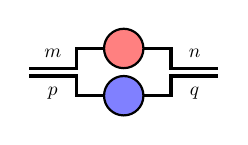
\begin{tikzpicture}[baseline=-0.5ex]
    \tikzset{tensor/.style = {minimum size = 0.5cm,shape = circle,thick,draw=black,inner sep = 0pt}, edge/.style   = {thick,line width=.4mm}}
    \def\x{0}
    \def\y{0}
    \node[tensor,fill=red!50!white] (A) at (\x,\y+0.3){$\Ab$};
    \node[tensor,fill=blue!50!white] (B) at (\x,\y-0.3){$\Bb$};
    \draw[edge] (\x-0.25,\y+0.3) -- (\x-0.6,\y+0.3) -- (\x-0.6,\y+0.05)   -- (\x-1.2,\y+0.05) node [midway,above] {\scalebox{0.7}{\dimcolor{$m$}}};
    \draw[edge] (\x-0.25,\y-0.3) -- (\x-0.6,\y-0.3) -- (\x-0.6,\y-0.05) -- (\x-1.2,\y-0.05) node [midway,below] {\scalebox{0.7}{\dimcolor{$p$}}};
    \draw[edge] (\x+0.25,\y+0.3) -- (\x+0.6,\y+0.3) -- (\x+0.6,\y+0.05) -- (\x+1.2,\y+0.05) node [midway,above] {\scalebox{0.7}{\dimcolor{$n$}}};
    \draw[edge] (\x+0.25,\y-0.3) -- (\x+0.6,\y-0.3) -- (\x+0.6,\y-0.05) -- (\x+1.2,\y-0.05) node [midway,below] {\scalebox{0.7}{\dimcolor{$q$}}};
\end{tikzpicture}
=\Ab \kron \Bb.
$$

